\documentclass{standalone}

\usepackage{tikz}
\usepackage{circuitikz}

\tikzset{block/.style = {draw, fill=white, very thick, rectangle, minimum height=1cm, minimum width=2cm},
         lblock/.style={draw,fill=white,very thick, rectangle, minimum height=3cm, minimum width=1cm},
         sum/.style= {draw, fill=white, very thick, circle, node distance=0.5cm}}

         
\begin{document}
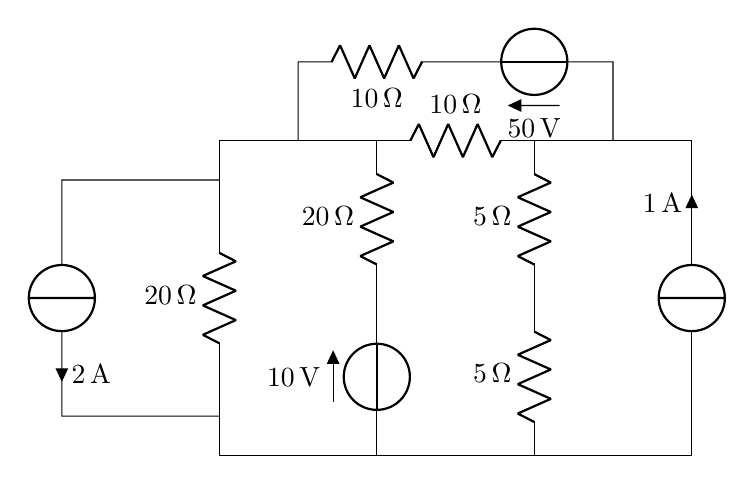
\begin{tikzpicture}
    \draw (0,0) to[R=$20\,\Omega$] (0,4)
                to[short](2,4)
                to[R=$10\,\Omega$](4,4)
                to[short](6,4);
    \draw (0,0) to[short](6,0);
    \draw (2,0) to[european voltage source=$10\,\mathrm{V}$](2,2)
                to[R=$20\,\Omega$](2,4);
    \draw (4,0) to[R=$5\,\Omega$] (4,2)
                to[R=$5\,\Omega$](4,4);
    \draw(0,3.5)to[short] (-2,3.5)
                to[european current source=$2\,\mathrm{A}$](-2,0.5)
                to[short](0,0.5);
    \draw (5,4) to[short](5,5)
                to[european voltage source=$50\,\mathrm{V}$](3,5)
                to[R=$10\,\Omega$](1,5)
                to[short](1,4);
    \draw (6,0) to[european current source=$1\,\mathrm{A}$](6,4);

\end{tikzpicture}
\end{document}